\chapter{INFORMATION PROPAGATION AND VIRALITY PREDICTION} \label{sec:2}

\let\thefootnote\relax\footnotetext{
Portions of this chapter previously appeared as:}
\let\thefootnote\relax\footnotetext{X. Lu, and B.~K. Szymanski, ``Towards limited scale-free topology with dynamic peer participation,'' {\em Computer Networks}, 2016.
}
\let\thefootnote\relax\footnotetext{
X. Lu, and B.~K. Szymanski, ``Predicting viral news events in online media,'' {\em IEEE International Parallel and Distributed Processing Symposium Workshops}, 2017.
}
\let\thefootnote\relax\footnotetext{
X. Lu, and B.~K. Szymanski,
``Scalable prediction of global online media news virality,'' {\em IEEE Transactions on Computational Social Systems}, 2018.}


%%% INTRODUCTION
\section{Introduction}
With the rise of online medium sites such as Facebook and Twitter, information propagation in these platforms attracts the interests of many researchers. Understanding the information propagation in these systems does not only provide better insights into the underlying sociology but is also crucial for the prediction of emergent social, economic and political phenomena. In the previous section, we study the detection of community structures in the complex network. In contrast, here, based on the topological features, we seek to predict the virality of cascades over the information propagation networks.

The mutual excitations between network nodes are widely observed in a variety of networks, ranging from the diffusion of purchasing behavior among friends to the spread of contagious disease. In a social network, information propagation can also be explained by the mutual excitations between individuals. Many previous works~\cite{weng2014predicting,zhao2015seismic,guille2012predictive} model the information diffusion as epidemics on networks - the acceptance of information is viewed as an infection of a node by infected neighbors in the network. These works assume that there exists an explicit propagation pathway which is sufficient to explain the observed information diffusion~\cite{yang2015defining} - messages can only spread along the predefined edges between nodes. In this section, we adopt these assumptions and develop efficient algorithms to predict the viral information propagation at its early stage.

As shown in~\cite{nematzadeh2014optimal}, strong community structures in a network enhance the local, intra-community spreading. This phenomenon is supported by the observations in online media: most news events are reported by the online news sites in the same region, using the same language. We exploit such community structures to parallelize the derivation of node embeddings because most cascades occur in local communities. In Section~\ref{sec:3.2}, according to the frequency of co-occurrence in cascades, the nodes in a network are divided into multiple communities in which the propagation occurs frequently. Every node in the propagation network has two latent vectors, one representing its influence to other nodes on different topics and the other representing its selectivity upon the inputs from other nodes on different subjects~\cite{bogdanov2014modeling}. Such latent representations of the influence and selectivity are analogous to the node's vector representation in the non-negative matrix factorization approach~\cite{lee2001algorithms,psorakis2011overlapping,yang2013overlapping}, where the inner product of two vectors indicates the strength of the connection between the corresponding nodes. These node embeddings are then used as input to predict the size of cascades. Unlike~\cite{gomez2013structure}, we represent the possible parameters of one link by the influence and selectivity of its two endpoints, which reduces the number of possible parameters and permits an efficient parallel algorithm to infer them. 

In Section~\ref{sec:3.2}, we propose a scalable community-based probabilistic framework to model the spreading of news about events in online media. News reports shape the public perception of the critical social, political and economic events around the world. The way in which emergent phenomena are reported in the news makes the early prediction of such phenomena a challenging task. Our approach exploits the latent community structure in the global news media and uses the affiliation of the early adopters with a variety of communities to identify the events widely reported in the news at the early stage of their spread. The time complexity of our approach is linear in the number of news reports. It is also amenable to efficient parallelization. To demonstrate these features, the inference algorithm is parallelized for message passing paradigm and scales well on RPI Advanced Multiprocessing Optimized System (AMOS), one of the fastest Blue Gene/Q supercomputers in the world. Thanks to the community-level features of the early adopters, the model gains an improvement of 20\% in the early detection of the most massively reported events compared to the feature-based machine learning algorithm. Its parallelization scheme achieves orders of magnitude speedup.

The scale-free topology has some good properties to facilitate information propagation, including high tolerance to random attacks\cite{albert2000error}, high synchronizability\cite{korniss2007synchronization} and resistance to congestion\cite{toroczkai2004network}. For this reason, several growth models are proposed to construct the scale-free overlay topology. The BA model\cite{barabasi1999emergence} manages to explain the evolution of scale-free topologies by a core principle named ``Preferential Attachment'' which means a new node is more likely to connect to heavily linked nodes when it joins the network. However, it is not practical in real distributed applications because the global information is required to maintain the degree distribution. Therefore, a distributed approach that constructs the topology without global information is desired.

In Section~\ref{sec:3.3}, we propose a distributed algorithm to construct limited scale-free networks which are robust against the traffic congestion and network failures~\cite{lu2016towards}. We compare our approach with other P2P network construction algorithms including HAPA\cite{guclu2009limited}, Gaian\cite{bent2008dynamic} and SRA\cite{bulut2014constructing} algorithms which construct the scale-free overlay topology with partial or no global information. The results show that our approach can maintain a scale-free overlay network while the other approaches are often vulnerable to dynamical peer participation. 

\section{Scalable prediction of global online news} \label{sec:3.2}

\subsection{Datasets} \label{sec:3.2.1}
We investigate the news data in the Global Database of Events, Language, and Tone (GDELT)\footnote{http://www.gdeltproject.org/} project. The GDELT project provides real-time news events extracted from tens of thousands of online news sites around the globe. Advances in natural language processing allows the sentiment analysis, real-time translation of 65 languages and the identification in events data of named entities including organization, location, count and theme. The dataset is currently available on Google Cloud Platform. Users can use Google BigQuery to download specific tables or process the data remotely by SQL commands. The GDELT database contains records the mentions of news events by news sites since February 19, 2015 to present. Here we present some unique features explored in these records. 

\begin{itemize}
\item \textbf{Emergence of news events}.
We calculate the duration of events, computed as the period since its earliest record until the latest. Most news events are reported by the news site within the first 50 hours. This reflects the short life cycle of the production and consumption of the news events. One explanation for this phenomenon is that a news site would prefer not to report an event which is considered out-of-date. In contract to the breaking news, the discussion of long-term topics such as greenhouse effect lasts a very long time, but these events constitute a very small portion of the dataset.

\begin{figure}[t!]
\centering
\begin{subfigure}{.5\textwidth}
\centering
\includegraphics[width=.99\linewidth]{img/chap3/dendro.pdf}
\caption{Dendrogram of hierarchical clustering of the 5,000 random cascades of news events} \label{fig:dendro}
\end{subfigure}
\begin{subfigure}{.45\textwidth}
\includegraphics[width=.99\linewidth]{img/chap3/news_sites_graph.pdf}
\caption{Backbone network of the news sites associated with the 5,000 sampled cascades of news events} \label{fig:backbone}
\end{subfigure}

\caption{The hierarchical structure of online media and the backbone co-reporting network.}
\end{figure}

\item \textbf{Most cascades are local}. 
For a period covering one year, we randomly choose 5,000 news events in the GDELT dataset. Any two news sites reporting at least 50 events together are linked in the graph shown in Figure~\ref{fig:backbone}. Clearly, there are four clusters visible in Figure~\ref{fig:dendro}, one standing for the news sites in the U.S., one for the news sites in Australia and the other for the news sites in European countries, while the remaining one is a mixture of sites in different regions. Initially, the pair-wise distance between any two cascades of events is measured by the Jaccard-index
\begin{equation}
    \text{Jaccard} = \frac{|N(i)\cap N(j)|}{|N(i)\cup N(j)|}
\end{equation}
where $N(j)$ is the set of news sites reporting the news event $j$. Then the hierarchical clustering algorithm~\cite{johnson1967hierarchical}, which merges iteratively the closest cascades according to the Ward distance measure among all pairs of cascades, is applied to obtain a dendrogram as shown in Figure~\ref{fig:dendro}. The Ward distance and the number of cascaded contained in a cluster are also plotted in text at some associated inner nodes of the clustering tree. There are three obvious clusters shown in the dendrogram. The largest cluster in blue corresponds to the news sites in the U.S., while most news sites in Australia are located in the middle cluster in green. The news sites in U.K. and European countries are placed in the left-most cluster in red. Although the plot shows only a raw distribution of the news site in different clusters, the dual visualization indicates that the hierarchical structures of cascades correlate with the community structure of co-reporting networks of the news sites. That is, as an illustrative example here, most cascades of news events occur frequently within certain regions only.

\item \textbf{Matthew effect in online media}.
The term  Matthew effect (or accumulated advantage) originated in sociology and refers to a phenomenon in which ``the rich get richer and the poor get poorer.'' In network science, it refers to preferential attachment of earlier nodes in a network~\cite{barabasi1999emergence} where nodes that few nodes that acquire more connections than others will increase its connectivity at a higher rate while others have few connections. As seen in Figure~\ref{fig:popularity}, the distribution of the number events reported per site follows the Power Law, which has been widely observed in a variety of networks. As shown in Figure~\ref{fig:popularity}, only a few popular news sites have reported millions of events, while most of the news site reported 5,000-10,000 events. In the Figure~\ref{fig:popularity}, the news site which reported less than 5,000 events in one year are ignored because they are less influential than the remaining ones. The goodness-of-fit is measured by the p-value as shown in Figure~\ref{fig:popularity_pvalue}.

\begin{figure}
\includegraphics[width=0.46\textwidth]{img/chap3/histo.png}
\centering
\caption{The distribution of the number of events reported by the news sites follows the power law.}\label{fig:popularity}
\end{figure}

\begin{figure}
\includegraphics[width=0.46\textwidth]{img/chap3/histo_pvalue.png}
\centering
\caption{Goodness of fit measured by the p-value}\label{fig:popularity_pvalue}
\end{figure}
\end{itemize}
    
We also generate \textbf{synthetic information cascades} to evaluate the performance of the prediction algorithms proposed in this section. The networks are generated using the Stochastic Block Models as discussed in Section~\ref{sec:2.2.2}. Given the membership of all the $n$ nodes, the edge with two endpoints in different communities is created with the probability $\beta$ and the edge inside a community is created with probability $\alpha$. In most cases, $\alpha$ is much larger than $\beta$, so the graph contains the dense intra-community structures and sparse  inter-communities structures. We create the SBM graphs containing 2,000 nodes with $\alpha=0.2$ and $\beta=0.001$. The average degree of nodes is approximately 10. Each community in SBM graph contains approximately $40$ nodes.

On each network instance, the spreading process is simulated according to the stochastic propagation model proposed by Kempe et al.~\cite{kempe2003maximizing}. Since any cascade would eventually flood the entire network, we set an observation window during for the cascades. After the observation window, the current spreading process will be terminated instantly and a random node is chosen as the initiator to start the simulation of the next cascade. A total of 3,000 cascades are collected for each graph instance. The first 2,000 cascades are used to infer the influence and selectivity vectors of nodes in the network and the last 1,000 cascades are used to test the accuracy of the virality prediction algorithm. For the last 1,000 cascades, the infections occurring in the first 2/7 time of the observation window are provided for the prediction task, while the remaining parts of infections are assumed to be unknown.

More formally, the infection delay of $v$, i.e. $t_v$, can be treated as a random value
\begin{equation}
\begin{array}{rcl}
   &t_v = \min{t_{u_1}, t_{u_1},\dots,t_{u_r}} \\
   &\forall i \in [1,r] \quad : \quad t_{u_i} \sim \mathcal{K}(\alpha_{u_i,v})
\end{array}
\end{equation}
where $t_{u_i}$ is the infection time of the $i$-th neighbors of node $v$, $\alpha_{u_i,v}$ is a parameter associated with the edge $(u,v)$ in the propagation network and $\mathcal{K}()$ is the distribution of infection delays. In our experiments, $\mathcal{K}()$ is set as the exponential distribution which is observed in many social dynamics~\cite{barabasi2005origin}, and we set $\forall (u,v)\in E$: $\alpha_{u,v}=1$ for simplicity. In theory, the IC model supposes the entire network will be infected given a sufficiently long period. Since contagions generally do not infect all the nodes in the network, in our experiments the simulation of every cascade happens within a predefined observation window~\cite{gomez2013structure}.

\subsection{Community affiliation model for information cascades}
Community structures are widely observed in a variety of networks. Based on patterns of news about events spreading in the online news media, we present two basic observations below: 
\begin{itemize}
    \item Most news sites have a preference for the topics of their news coverage, e.g. politics, finance, education, military, technology or sports.
    \item The news reports are usually confined to the geographical and cultural boundaries. Although many media companies have ambitions to have global market presence, most media sites have only a regional reach~\cite{hjarvard2001news}.
\end{itemize}

Much like many community detection methodologies \cite{blondel2008fast,clauset2004finding,lu2017adaptive,xie2011community,fortunato2010community} which aim at discovering dense sub-graphs embedded in a network, we seek to recover such community structure for the online news sites. However, in the global and local news markets~\cite{leetaru2013gdelt}, connecting every two sites reporting the same event could result in an extremely dense network. Finding community structure in such network would not only incur high computational power but would also cloud the real connections among communities. Therefore, we find the latent community affiliation of these news sites rather than drawing the edges between specific news sites. Since the underlying network topology is unknown, our probabilistic model incorporates the time points of each infection in the observed news cascades, i.e., the time of each news report. Formally, we present the definition of information cascade below.

An information/news cascade is a set of infections $\{(u, t_u)\}$. Each infection $(u, t_u)$ consists of a node $u$ and its infection time $t_u$. Our model assumes the news cascades happen at the community level. For a particular community of news sites, the probability of a site reporting a particular news depends on both the affiliation of this news sites with the community and the probability of the news cascade reaching its community. To formalize this idea, we define latent community below.

A latent community is a set of nodes that, conditioned on the infection of one member, the probability that other members will get infected within a limited period is much higher than for the non-members. In \cite{yang2013overlapping}, authors propose a community affiliation model where each node has a probability belonging to one of the overlapping communities in the network. We extend this community affiliation model by taking into account the probability for each cascade to spread to these overlapping latent communities. As illustrated in Figure~\ref{fig:affiliation_model1}, if a cascade has a non-zero probability of spreading to a community, this cascade (square) is connected to the community (double circle); if a node (circle) belongs to a community, then this node is connected to the community as well. Our affiliation model captures two important features of cascades and communities in complex networks: (i) the community structures are highly overlapped, a node can belong to multiple communities at the same time; (ii) the members of the same community tend to accept similar information during the information cascades. 

\begin{figure}
\includegraphics[width=.6\textwidth]{img/chap3/affiliation_model_V2.pdf}
\centering
\caption{Community affiliation model with cascades. Cascade $c$ belongs to the two leftmost communities, and node $u$ belongs to community $i$.}\label{fig:affiliation_model1}
\end{figure}

Social theories~\cite{barabasi2005origin} suggest that the response time of human beings usually follows the exponential distribution, which explains the burstiness of social behavior in many scenarios. Our analysis of 723,037 randomly sampled news reports shows that the delays of news reports also fit the exponential distribution with a high $R^2$ score of 92\%. We consider the news reports with a delay less than 21 hours, which comprise 99\% of the sampled data from the Global Database of Events, Language, and Tone (GDELT) dataset. Based on this observation, we model the response time of news sites to events by an exponential distribution.

For every single community $i$, let $A_{ui} > 0$ denote the strength of affiliation of node $u$ with it and $M_{ci} \in (0,1]$ denote the probability of the cascade spreading to community $i$. In this community, the response time of node $u$ to cascade $c$ follows the exponential distribution
\begin{equation} \label{eq:expo_ez}
t_u^c(i) \sim Exp(A_{u,i} M_{c,i})
\end{equation}
which indicates that the node $u$ gets quickly infected when the cascade $c$ is highly likely to reach a community $i$, i.e. $M_{c,i}$ is large, and the affiliation of $u$ with community $i$ is strong, i.e. $A_{u,i}$ is large.

Most real-world networks have overlapping community structures which allow a node to belong to many communities. Therefore, in our model, the response time of a node to a cascade corresponds to the minimum response time in all communities. Given a node $u$, a cascade $c$ and a total of $m$ overlapping communities, the minimum response time also follows the exponential distribution\footnote{The minimum of $m$ mutually independent random variables $X_i \sim Exp(\lambda_i)$ for $i=1,2,\dots,m$ also follows the exponential distribution, i.e. $min(X_i) \sim Exp(\sum_i\lambda_i)$.} 

\begin{equation} \label{eq:total}
\min \{ t_u^c(1),t_u^c(2),\dots, t_u^c(m) \} \sim  Exp(\sum_{i=1}^{m} A_{u,i} M_{c,i} ) 
\end{equation}
where the rate parameter is the sum of the rate parameters for each individual exponential distribution in Eq.~\ref{eq:expo_ez}.

In reality, news agencies usually have some bias for the content of information they spread. Such bias can be positive - there are certain types of information a news agency favors, while it can also be negative - messages of no interest to agency's audience are ignored or intentionally blocked. It is tempting to allow the value of $M_{c,i}$ to be negative for this reason so that the affiliation with some community may delay the response time of some node, i.e. $A_{c,i} M_{c,i} < 0$. However, it could result in a negative rate parameter $\lambda$ in Eq.~\ref{eq:total} which violates the constraint $\lambda > 0$ of the exponential distribution. Hence, we smooth the rate parameter via the sigmoid function $\sigma : \mathbb{R} \to [0,1]$. In this way, given an information cascade $c$, the response time of a node $u$, $t_u^c = \min  t_u^c(i)$, draws from an exponential distribution with a rate parameter $\gamma = w \sigma( A_u \cdot M_c)$,
\begin{align} \label{eq:sigmoid}
t_u^c \sim Exp(w \sigma(A_u \cdot M_c))
\end{align}
where $\sigma(x)= \frac{1}{1+e^{-x}}$ is the sigmoid function, $w$ is a scaling parameter and $\cdot$ represents the inner product in vector space, while the $i$-th component of vector $A_u$ and $M_c$ are  $A_{ui}$ and $M_{ci}$ respectively. Using the sigmoid function here avoids any constraint for the parameters $A_u$ and $M_c$, and most importantly, it improves the robustness of the parameter estimation because the sigmoid function is differentiable at each point. 

So far, the model takes into account the participants of a cascade. However, the nodes which are not involved in a cascade also provide information about their affiliations with different communities. Since these silent nodes are equivalently important, we set a upper bound on the response time, $T \gg t_u^c $ for $\forall u$ and $\forall c$, such that all the silent nodes during the cascading propagation can be assumed to have this long response time $T$.

Given an information cascade $c=\{(u_i^c, t_i^c) | i=1,2,\dots,n_c\}$ where the $i$-th node $u_i^c$ has response time $t_i^c$, the likelihood of observing a cascade $c$ is
\begin{equation} \label{eq:casc_likelihood}
L_c = \prod_{u\in V_c} p_{u,c}(t_u^c)  \prod_{u \notin V_c}  p_{u,c}(T)
\end{equation}
where $V_c = \{u_i^c | i=1,2,\dots,n_c\}$ denotes the set of nodes involved in cascade $c$ and $p_{u,c}(t)$ is the probability density function of the exponential distribution
\begin{equation} \label{eq:pdf}
p_{u,c}(t) = w\sigma( A_{u} \cdot M_c) e^{-w\sigma( A_{u} \cdot M_c) t}
\end{equation}
Since the likelihood $L_c$ is the product of $|V|$ terms, Eq.~\ref{eq:casc_likelihood} can be too expensive to compute. But it can be approximated by using a subset of representatives $D_c$ drawn randomly from $V\setminus V_c$. This idea is similar to the negative sampling approach~\cite{mnih2012fast}, which has been successfully applied to learning the distributed representation of words in documents~\cite{mikolov2013distributed,ji2016parallelizing}. The log-likelihood of an observed cascade then becomes
\begin{equation} \label{eq:neg}
\begin{array}{rcl}
   \mathcal{L}_c \approx & \sum_{u \in V_c} \log p_{u,c}(t_u^c) + \sum_{u\in D_c} \log p_{u,c}(T)
\end{array}
\end{equation}
where $D_c$ is the set of negative samples chosen for every cascade by drawing random nodes uniformly from $V$. If we fix the size of each $D_c$ as $d$, then a speedup of approximately $|V|/d$ times can be achieved.

To estimate the parameters $A_u$ for each $u$ and $M_c$ for each $c$, we maximize the likelihood which factorizes into the product of the likelihoods of $k$ cascades. This goal is equivalent to maximizing the sum of the log-likelihood of $K$ cascades
\begin{equation} \label{eq:loglikelihood}
\{\hat{A}_u\}, \{\hat{M}_c\} = \argmax_{\{A_u\}, \{M_c\}} \sum_{c=1}^{k} \mathcal{L}_c
\end{equation}
It is worth noting that the problem defined by Eq.~\ref{eq:loglikelihood} does not require explicit network topology to estimate $A_u$ and $M_c$. Instead, the input of the model is the response times of the nodes to every cascade. This is a practical setting when the underlying network topology is incomplete or hidden during the information propagation process. In addition, the parameter space $\{A_{ui},M_{ci}|\forall i,u,c\}$ in Eq.~\ref{eq:loglikelihood} does not have any restriction thanks to the adoption of the sigmoid function in Eq.~\ref{eq:sigmoid}.

The optimization problem in Eq.~\ref{eq:loglikelihood} is unfortunately not convex. Since the network size can be large, the optimization problem involves a large number of parameters, which makes stochastic updates more suitable than the batch methods. In addition, when some new cascade data comes in, the estimation algorithm should be able to incorporate the new cascades efficiently. For these reasons, we apply the Stochastic Gradient Ascent (SGA) method to estimate the parameters.

If we substitute Eq.~\ref{eq:neg} into Eq.~\ref{eq:loglikelihood}, the partial derivative of the objective function $F$ in Eq.~\ref{eq:loglikelihood} over a particular $M_c$ becomes 
\begin{equation} \label{eq:partial}
    \frac{\partial F}{\partial M_c} =  \sum_{u\in V_c} \frac{\partial \log p_{u,c}(t^c_u) }{\partial M_c} + \sum_{u\in D_c} \frac{\partial \log p_{u,c}(T) }{\partial M_c}
\end{equation}
which is a weighted sum of the terms in the form of $\frac{\partial \log p_{u,c}(t) }{\partial M_c}$. Given the value of $t$, $p_{u,c}(t)$ depends only on $A_u$ and $M_c$. The partial derivative of $\log p_{u,c}(t)$ over $M_c$ can be computed using $A_u$ and $M_c$
\begin{equation} 
    \frac{\partial \log p_{u,c}(t)}{\partial M_c} = \big[1 - \sigma( A_u \cdot M_c) w t\big] \big[1-\sigma( A_u \cdot M_c)\big] A_u
\end{equation}
Here we need the $A_u$ for $\forall u \in V_c \cup D_c$ to update $M_c$ according to the gradient in Eq.~\ref{eq:partial}. Similarly, the partial derivative of the objective function $F$ in Eq.~\ref{eq:loglikelihood} over $A_u$ can be computed using the $M_c$ for cascades $c$ such that $u \in V_c \cup D_c$
\begin{equation}
\frac{\partial F}{\partial A_u} =  {\sum_{c:u\in V_c}} \frac{\partial \log p_{u,c}(t^c_u) }{\partial A_u} + {\sum_{c:u\in D_c}} \frac{\partial \log p_{u,c}(T) }{\partial A_u}
\end{equation}
where the term $\frac{\partial \log p_{u,c}(t)}{\partial A_u}$ depends on $A_u$ and $M_c$ only
\begin{equation} 
    \frac{\partial \log p_{u,c}(t)}{\partial A_u} = \big[1 - \sigma( A_u\cdot M_c) w t\big] \big[1-\sigma( A_u\cdot M_c)\big] M_c
\end{equation}
In this way, the parameters can be updated in a pair-wise manner: we fix $A_u$ for all $u$ and update all the $M_c$s, and then fix all $M_c$s to update $A_u$s in every SGA iteration. The SGA updates can operate on a bipartite graph where node $u$ and cascade $c$ are connected if $u\in V_c \cup D_c$ (cf. the example shown in leftmost diagram in Figure~\ref{fig:pll}). To update $A_{u}$, each cascade $c$ propagates the corresponding parameters $M_c$ through the links in the bipartite graph to the node $u$. Then node $u$ calculates the partial derivative $\frac{\partial \log p_{u,c}(t) }{\partial A_{u}}$ for every connected cascade $c$ and updates $A_{u}$ accordingly. Similarly, the nodes can propagate the parameters $A_u$s through the links in this bipartite graph towards each relevant cascade $c$, and $M_{c}$ can be updated using the $A_u$ it receives. 

The pseudo code is shown in Algorithm~\ref{algo:sga1}.
The \textbf{time complexity} of each SGA iteration here is linear in the number of edges in the bipartite graph. This is because the loop in lines 8-19 iterates over all the nodes $u$ connected with each cascade $c$, which corresponds to visiting every edge of the bipartite graph exactly once. Similarly, the lines 20-31 also visit every edge in the bipartite graph once. In the news dataset, the number of edges of the bipartite graph is defined by the number of news reports, because every report connects a news site to a news cascade, plus the pair of negative samples edges $(u, c)$ for $u\in D_c$ with $|D_c|=d$ fixed as a constant. Hence, the time complexity of each SGA iteration is linear in the number of edges in the bipartite graph. The time complexity of Algorithm~\ref{algo:sga1} is also determined by the number of SGA iterations. In practice, this only involves tens of iterations before the derived $A_u$ and $M_c$ vectors become stable. Thus, this number can be treated as a constant. Therefore, the Algorithm~\ref{algo:sga1} has a linear time complexity in the number of bipartite graph edges, i.e. the number of news reports.


\begin{algorithm}
\caption{SGA Algorithm using a Single Processor}\label{algo:sga1}
\begin{algorithmic}[1]
\State $\alpha = \text{the SGA stepsize}$
\For {each cascade $c$} 
\For {each node $u \in V_c$}
\State $t_u^c = \text{infection delay of node $u$ in cascade $c$}$
\EndFor
\EndFor
\For {each SGA iteration}
\For {each cascade $c$} 
\For {each node $u \in V_c \cup D_c$}
\If {$u \in V_c$}
\State $t= t_u^c$
\ElsIf{$u \in D_c$}
\State $t= T$
\EndIf
\For {$i = 1,2,\dots,m$}
\State $A_{ui} \pluseq \alpha \frac{\partial \log p_{u,c}(t) }{\partial A_{ui}}$
\EndFor
\EndFor
\EndFor
\For {each node $u \in V$}
\For {each cascade $c$ such that $u \in V_c \cup D_c$}
\If {$u \in V_c$}
\State $t= t_u^c$
\ElsIf{$u \in D_c$}
\State $t= T$
\EndIf
\For {$i = 1,2,\dots,m$}
\State $M_{ci} \pluseq \alpha \frac{\partial \log p_{u,c}(t) }{\partial M_{ci}}$
\EndFor
\EndFor
\EndFor
\EndFor
\end{algorithmic}
\end{algorithm}

\subsection{Parallelization for distributed memory machines}
In practice, the input network size can be large so to speed up computation we offer parallelization of the parameter estimation for our model. Since the SGA algorithm is inherently sequential, many works including~\cite{ji2016parallelizing,mikolov2013distributed} use the Hogwild! framework~\cite{recht2011hogwild} attempting to parallelize the SGA algorithm on shared memory machines. The Hogwild! framework ignores the write-write conflicts caused by parallel updates on the same parameter as long as one unique processor can complete its writing operation. The quality of the results produced by SGA algorithm is guaranteed by the property that such conflicts are sparse enough. In the information diffusion context, however, such data sparsity is uncertain. To handle the contentions between processors, we propose a scalable parallelization scheme based on message passing paradigm~\cite{gropp1999using}.

The parallelization scheme is illustrated in Figure~\ref{fig:pll}. Consider eight nodes (blue) involved in eight cascades (yellow) in this toy example. The bipartite graph connects every pair of associated nodes and cascades in the SGA updates. These nodes and cascades are then distributed in this example to two processors. The first processor owns the upper four nodes and upper four cascades while the remaining nodes and cascades are assigned to the second processor. Each processor creates private memory space for the parameters of the nodes and cascades it owns. Much like Algorithm~\ref{algo:sga1}, the SGA algorithm propagates parameters back and forth between nodes and cascades, the only difference here is that the propagation between the cascades and nodes owned by different processors requires inter-core communication.

During every SGA iteration, each node $u$ propagates its $A_u$ to all the connected cascades in the bipartite graph. If these cascades are located in the same processor which owns node $u$, then this propagation operation is done locally. Otherwise, $A_u$ is sent \textbf{asynchronously} to the processor owning node $u$. The pseudo code for the parallelization scheme is shown in Algorithm~\ref{algo:2} and Algorithm~\ref{algo:3}. Without loss of generality, we consider updating $M_c$s using $A_u$s, i.e. the line 14 in Algorithm~\ref{algo:2}. One SGA iteration consists of the following three phases:
\begin{itemize}
\item (a) Message passing: Every processor sends the $A_u$s it owns to the target processors which require those $A_u$s to update their corresponding $M_c$s, cf. the lines 1-3 in Algorithm~\ref{algo:3}.
\item (b) Local updates: Every processor updates the $M_c$ it owns using the gradients $\frac{\partial \log p_{u,c}(t) }{\partial M_{c}}$ if it also owns $A_u$, cf. the lines 4-6 in Algorithm~\ref{algo:3}. 
\item (c) Remote updates: After all the remote $A_u$s sent in phase (a) have been received, each processor updates $M_c$ using the gradients $\frac{\partial \log p_{u,c}(t) }{\partial M_{c}}$ whose computation requires some of the received $A_u$s, cf. the lines 8-10 in Algorithm~\ref{algo:3}.
\end{itemize}
Note that each processor should conduct the local updates prior to the updates which require remote data from other processors, i.e. the phase (b) occurs before the phase (c). In this way, the local computation time and inter-core communication time overlap with each other, improving the parallelization efficiency. 

\begin{figure}[t]
\includegraphics[width=.8\textwidth]{img/chap3/propagation_node_casc.pdf}
\centering
\caption{Illustration of the parallelization scheme using two processors. The parameters propagate back and forth between nodes and cascades iteratively. If the connected node and cascade are in the different processors, the parameters are sent via asynchronous communication, i.e. the blue dashed lines marked by ``ISend''. At the same time, the local parameter propagation occurs within each processor, i.e. the bold black arrows in the middle. This figure illustrates the parameter propagation from node layer to cascade layer. The parameter propagation from cascade layer to node layer is conducted in a similar manner.}\label{fig:pll}
\end{figure}
\begin{algorithm}
\caption{Parallelized SGA Algorithm (Distributed Memory Machines)}\label{algo:2}
\begin{algorithmic}[1]
\For {each cascade $c$}
\State $proc(c) = $ ID of the processor storing $M_c$
\EndFor
\For {each node $u$}
\State $proc(u) = $ ID of the processor storing $A_u$
\EndFor
\ForAll {each processor $p$ {\bf in parallel}}
\State $U_p = $ IDs of the nodes owned by processor $p$
\State $C_p = $ IDs of the cascades owned by processor $p$
\EndFor
\For {each SGA iteration}
\ForAll {each processor $p$ {\bf in parallel}}
\State Call Algorithm~\ref{algo:3} to update $M_c$s using $A_u$s
%\LineComment{Update $A_u$s using $M_c$s}
%\LineComment{Update $A_u$s using $M_c$s}
\EndFor
\ForAll {each processor $p$ {\bf in parallel}}
\State Call Algorithm~\ref{algo:3} to update $A_u$s using $M_c$s similarly
%\LineComment{Update $A_u$s using $M_c$s}
%\LineComment{Update $A_u$s using $M_c$s}
\EndFor
\EndFor
\end{algorithmic}
\end{algorithm}

\begin{algorithm}
\caption{Parallelized SGA Updates of $M_c$s using $A_u$s (Distributed Memory Machines)}\label{algo:3}
\begin{algorithmic}[1]
%\State \COMMENT{\it 1.a Message passing}
\For {each $(u,c)$ s.t. $u \in U_{p}$, $c \notin C_p$ and $u \in V_c \cup D_c$}
\State Send $A_u$ to $proc(c)$ asynchronously
\EndFor
%\State \COMMENT{\it 1.b Local updates}
\For {each $(u,c)$ s.t. $u \in U_{p}$, $c \in C_p$ and $u \in V_c \cup D_c$}
\State Call Algorithm~\ref{algo:sga1} to update $M_c$ using $A_u$.
\EndFor
\State Wait for asynchronous receive requests until done
%\State \COMMENT{\it 1.c Remote updates}
\For {each $(u,c)$ s.t. $u \notin U_{p}$, $c \in C_p$ and $u \in V_c \cup D_c$}
\State Call Algorithm~\ref{algo:sga1} to update $M_c$ using $A_u$.
\EndFor
\end{algorithmic}
\end{algorithm}

Figure~\ref{fig:pll} illustrates this parallelization scheme. The three phases described above are represented by the three diagrams following the first diagram showing the initial stage in Figure~\ref{fig:pll}. The parameters propagate back and forth between node layer and cascade layer iteratively. If the connected node and cascade are in the different processors, the parameters are sent via asynchronous communication, i.e. the blue dashed lines labeled ``ISend''. At the same time, the local parameter propagation occurs within each processor, as indicated by the bold black arrows in the middle. Using the same protocol, we can update $A_u$s using the values of $M_c$s.

After distributing nodes and cascades to the processors, each processor creates its private memory space for the $A_u$s and $M_c$s it owns and ghost memory space for those $A_u$s and $M_c$s connected to the nodes or cascades in the bipartite graph, but owned by other processors. In every SGA iteration, once the ghost memory is filled with the received data, it will not be written again. For example, a processor owns two nodes $u$ and $v$, both involved in a cascade $c$ which is owned by another remote processor. To update $A_u$ and $A_v$, $M_c$ is sent asynchronously to this local processor. But $M_c$ will be sent only once regardless of the number of associated nodes owned by the local processor, because $M_c$ can be shared by the updates of $A_u$ and $A_v$. This optimization is similar to the combiner applied to the message queues in Pregal-like parallel graph processing systems~\cite{malewicz2010pregel,avery2011giraph} to avoid sending duplicated messages to the same target processor.

We test our parallelization scheme on RPI Advanced Multiprocessing Optimized System (AMOS), which is a 5-rack, 5K nodes, 80K cores IBM Blue Gene/Q system~\cite{haring2012ibm} with additional equipment. In AMOS supercomputer, each node consists of a 16-core, 1.6 GHz A2 processor, with 16 GB of DDR3 memory. Considering the fact that the inter-core communication is generally more efficient inside the same node than across different nodes, we use all the 16 cores of a node so that the communication between cores can be more efficient. In general, the maximum number of cores per node here is not constrained by the limit of 16 GB DDR3 memory space. This is one benefit of our memory management paradigm because every processor stores only one copy of the parameters of nodes and cascades associated with it.

\begin{figure}[t]
\centering
\begin{tabular}{c}

\begin{subfigure}{.45\textwidth}
\centering
\includegraphics[width=.99\linewidth]{img/chap3/Speedup_SBM_v1_D100.pdf}
\caption{m=100}\label{fig:Speedup_SBM_v1_D100}
\end{subfigure} 
\begin{subfigure}{.45\textwidth}
\centering
\includegraphics[width=.99\linewidth]{img/chap3/Speedup_SBM_v1_D200.pdf}
\caption{m=200}\label{fig:Speedup_SBM_v1_D200}
\end{subfigure} 

\end{tabular}
\caption{Speedup and efficiency of our parallelization scheme on Advanced Multiprocessing Optimized System (AMOS). $m$ denotes the dimension of $A_u$ and $M_c$.}
\label{fig:speedup_efficiency}
\end{figure}

%SBM_v1.txt 20K nodes, 10K cascades
The speedup and efficiency of our parallelization scheme are shown in Figure~\ref{fig:speedup_efficiency}. A total of 10K cascades are simulated on the SBM network with 20K nodes. Each cascade infects a total of 247 nodes on average. The Figure~\ref{fig:speedup_efficiency} shows that the parallelization scheme achieves an approximately linear speedup using several hundreds of processors. And the efficiency of the parallelization scheme is above 25\% in all cases. The comparison between Figure~\ref{fig:Speedup_SBM_v1_D100} and Figure~\ref{fig:Speedup_SBM_v1_D200} shows that the dimension $m$ does not change the speedup or efficiency. In our sampled GDELT dataset, the parallelized algorithm achieves the similar speedup and efficiency using 64 processors, but adding extra processors does not significantly increase the speedup due to the limited size of the dataset.

To test the scalability of the parallelization scheme, we evaluate the execution time of one single SGA iteration of Algorithm~\ref{algo:2} using 512 processors. Given a network of 10K nodes and the different numbers of cascades, Figure~\ref{fig:node_number_time} shows that the execution time is approximately proportional to the number of cascades. A similar pattern is also observed as the dimension $m$ grows. In contrast, when the number of cascades is fixed and the number of network nodes increases, the execution time grows slowly - the execution time only doubles when the number of network nodes grows from 5K to 20K. The reason is that the number of infections per cascade is relatively stable in the synthetic data so that the increase of time for parameter propagation is actually smaller than the increase in the number of network nodes. In general, the parallelization scheme scales well with the number of network nodes, the number of cascades and the dimension $m$.

\begin{figure}[t]
\centering

\begin{subfigure}{.45\textwidth}
\centering
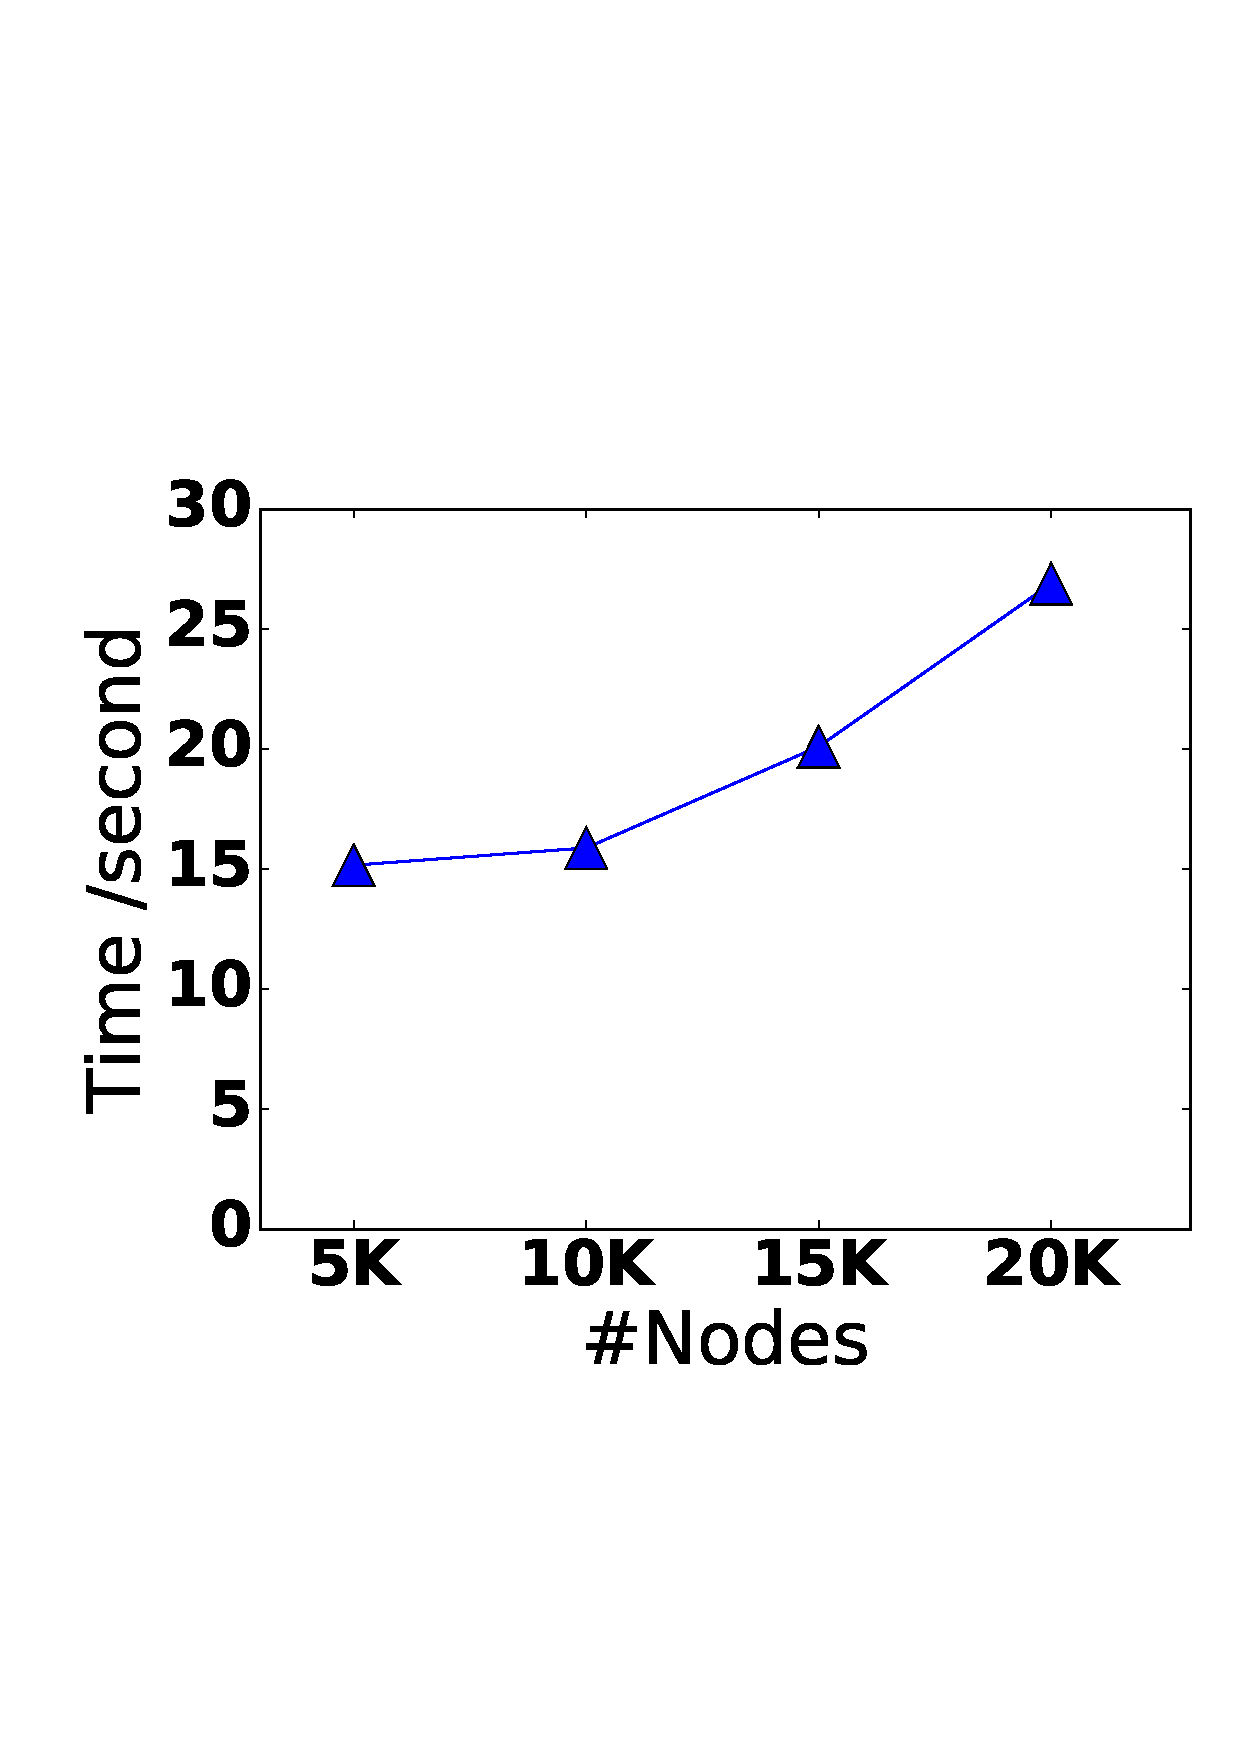
\includegraphics[width=.99\linewidth]{img/chap3/node_number_time.pdf}
\caption{m=200}\label{fig:node_number_time}
\end{subfigure} 
\begin{subfigure}{.45\textwidth}
\centering
\includegraphics[width=.99\linewidth]{img/chap3/cas_number_time.pdf}
\caption{m=200}\label{fig:cas_number_time}
\end{subfigure} %
\hfill

\begin{subfigure}{.45\textwidth}
\centering
\includegraphics[width=.99\linewidth]{img/chap3/dimension_time.pdf}
\caption{m=200}\label{fig:dimension_time}
\end{subfigure} 

\caption{The execution time of one SGA iteration in relation to the dimension $m$, the number of network nodes and the number of cascades.}
\end{figure}

\begin{table*}[ht]
\caption{Accuracy of the news virality prediction measured by F1 scores. The predictions of our proposed model (ML) are consistently better than the the baseline model's (BL) using the same set of early adopters in the first 30 to 60 minutes.}
\centering
\label{tab:onehour}
\begin{tabular}{|c|c|c|c|c|c|c|c|c|c|c|}
\hline
\multirow{2}{*}{Threshold $\theta$} & \multicolumn{2}{c|}{$\tau=$0.5 Hour} & \multicolumn{2}{c|}{$\tau=$0.6 Hour} & \multicolumn{2}{c|}{$\tau=$0.7 Hour} & \multicolumn{2}{c|}{$\tau=$0.8 Hour} & \multicolumn{2}{c|}{$\tau=$0.9 Hour} \\ \cline{2-11}
& BL & ML & BL & ML & BL & ML & BL & ML & BL & ML \\
\hline 
\hline
90\% &  0.410 & 0.500 & 0.410 & 0.497  & 0.410 & 0.499  & 0.499 & 0.549  & 0.499 & 0.548   \\  
\hline
91\% &  0.412 & 0.484 & 0.405 & 0.486  & 0.405 & 0.480  & 0.484 & 0.534  & 0.490 & 0.536   \\
\hline
92\% &  0.389 & 0.473 & 0.394 & 0.472  & 0.392 & 0.471  & 0.463 & 0.530  & 0.463 & 0.531   \\
\hline
93\% &  0.294 & 0.455 & 0.296 & 0.453  & 0.294 & 0.453  & 0.434 & 0.516  & 0.436 & 0.511   \\
\hline
94\% &  0.207 & 0.433 & 0.209 & 0.433  & 0.213 & 0.436  & 0.393 & 0.489  & 0.393 & 0.491   \\
\hline
95\% &  0.191 & 0.404 & 0.191 & 0.409  & 0.195 & 0.408  & 0.352 & 0.465  & 0.347 & 0.462   \\
\hline
96\% &  0.147 & 0.393 & 0.141 & 0.389  & 0.147 & 0.389  & 0.287 & 0.438  & 0.285 & 0.442   \\
\hline
97\% &  0.114 & 0.360 & 0.116 & 0.366  & 0.113 & 0.361  & 0.233 & 0.402  & 0.232 & 0.407   \\
\hline
98\% &  0.097 & 0.311 & 0.091 & 0.316  & 0.097 & 0.316  & 0.160 & 0.365  & 0.166 & 0.357   \\
\hline
99\% &  0.119 & 0.288 & 0.107 & 0.292  & 0.104 & 0.279  & 0.148 & 0.326  & 0.148 & 0.324   \\
\hline
\end{tabular}
\end{table*}


\subsection{Virality prediction via early adopters} \label{sec:forecast}
Our aim is to forecast the viral information cascade. From the historical cascades, the proposed model estimates the $A_u$ vector for each $u$ according to the observed response times. Using these $A_u$ vectors of the initially infected nodes, we seek to predict the behavior of future cascades.

Suppose a set of so-called early adopters have been infected within a limited time period. One basic observation is that, once the contagion reaches a community member, the probability that other members get infected increases. Therefore, we can make use of the infected node's local neighborhood to predict the infection future. Since our model presents every node $u$ by a vector $A_u$ in the latent space, it is easy to find the neighbors which are close to node $u$ by measuring the Euclidean distances between them. As the contagion is likely to spread fast in the dense areas, the number of neighbors within a certain range can be used as an indicator of future infections. Hence, we count the number of neighbors that are located within a certain range from the infected node $v$, and arrange these values in a vector $K$ whose $i$-th component is defined as
\begin{equation} \label{eq:prediction_}
K_i = |\{u|\|A_u - A_v\|_2 < r_i\}|
\end{equation}
where $r_i$ is the radius of the $i$-th neighborhood of node $v$ and $\|\cdot \|_2$ denotes the Euclidean norm.

Figure~\ref{fig:hood} demonstrates how to compute the $K$ vector of an infected node. Suppose the infected nodes are located at the centers of the different circles. Their neighborhoods are marked by the circles which have the radii $r_1$, $r_2$ and $r_3$ respectively. In Figure~\ref{fig:hood}, the node at the right center has 3 neighbors inside the small circle, 7 neighbors inside the medium circle and 12 neighbors inside large circle, resulting in the vector $K=[3,7,12]$. The leftmost node has only 1 neighbor, i.e. itself, inside both the small and medium circle and 5 neighbors inside the large circle, resulting in the vector $K'=[1,1,5]$. Intuitively, we can tell from $K$ and $K'$ that the right three neighborhoods allow faster growth of infections than the left ones. 

Given a set of early adopters which get infected within a limited time period, we can count the total number of \textbf{unique} neighbors in their local neighborhoods within different radii similarly. Note that if a node is in the $i$-th neighborhood of two early adopters, this node is only counted once in the $i$-th component of $K$. Finally, The numbers of neighbors, presented as the components of a multiple-dimensional vector $K$, are fed to a machine learning model to predict the final size of a cascade.

\begin{figure}
    \centering
    \includegraphics[width=.7\textwidth]{img/chap3/hood.pdf}
    \caption{Illustration of the local neighborhoods in the vector space. The concentric circles mark the neighborhoods with different radii from the center. The proposed method counts the number of nodes located in each circle and arrange these values in a vector. Vector $K$ shows the numbers of nodes for $r_1$, $r_2$ and $r_3$ radii drawn from the figure center while $K'$ is shown for the circles centered at the asterisk on the left.}
    \label{fig:hood}
\end{figure}

Our model produces the $A_u$ vector for each node $u$ in the network. If these $\{A_u\}$ vectors preserve the community structures of the news media network well, their clustering should match the community structure embedded in the explicit network topology, because the members of a community have similar $A_u$s.

Given a synthetic SBM network, we simulate the cascades as described in Section~\ref{sec:3.2.1}. Our model then infers the $\{A_u\}$ vectors by these cascades. For clarity, the set of nodes detected in a network is called a community and the set of nodes clustered by their vector representations is called a cluster here. We compare the node clustering of these $\{A_u\}$ vectors with the ground truth partition of the SBM network and the community structures discovered by traditional community detection algorithms from the explicit topology. The alignment between them indicates the $\{A_u\}$ vectors produced by our model preserve the community structures.

More specifically, the K-means clustering algorithm~\cite{macqueen1967some} is executed on the so-inferred $\{A_u\}$ vectors to derive the node clustering. The similarity between the node clustering and the contrastive partitioning of the network are measured by the Adjusted Mutual Information (AMI) and Adjusted Rand Score (ARS) which are widely used to evaluate community detection performance. Section~\ref{sec:2.2.3} presents the mathematical definitions of both metrics.

\begin{figure}
    \centering
    \includegraphics[width=.8\textwidth]{img/chap3/converge.png}
    \caption{The similarity between the node clustering of the $\{A_u\}$ vectors at each SGA iteration of Algorithm~\ref{algo:sga1} and the ground truth partition of the SBM network.}
    \label{fig:alignment_figure}
\end{figure}

\begin{table}[]
\caption{The pairwise similarities between the communities detected by the state-of-the-art community detection algorithms, the node clustering of the $\{A_u\}$ vectors produced by our model and the ground truth partition of the SBM network. The entries below and above the main diagonal represent the Adjusted Rand Score (ARS) and Adjusted Mutual Information (AMI) respectively. FG: Fast Greedy algorithm~\cite{clauset2009power}, LE: leading eigenvector method~\cite{newman2006finding}, LP: label propagation algorithm~\cite{raghavan2007near}, ML: multilevel algorithm~\cite{blondel2008fast}. Our model produces node embeddings whose clustering aligns well with the ground truth communities, even outperforming some community detection baseline methods.}\label{tab:alignment_table}
    \centering
    \begin{tabular}{|c|cccccc|}
   \hline
    ARS / AMI & FG & LE & LP & ML &  Our Model &  Ground Truth\\
   \hline
FG &  & 0.858 & 0.833 & 0.943 & 0.881 & 0.933 \\
LE & 0.873 &  & 0.807 & 0.867 & 0.795 & 0.837 \\
LP & 0.864 & 0.829 &  & 0.835 & 0.773 & 0.804 \\
ML & 0.929 & 0.881 & 0.868 &  & 0.922 & 0.949 \\
Our Model & 0.869 & 0.820 & 0.817 & 0.936 &  & 0.930 \\
Ground Truth & 0.939 & 0.865 & 0.852 & 0.963 & 0.925 & \\
\hline
    \end{tabular}
\end{table}

Figure~\ref{fig:alignment_figure} shows the growth of the similarity between the node clustering of the $\{A_u\}$ vectors at each SGA iteration and the ground truth partition of the SBM network. The SBM network has 100 nodes and 5 communities of size 20, 190 edges connects nodes in the same community and 12 edges are across different communities. A total of 100 cascades are simulated, each involves 12.5 infections on average. The dimension of $A_u$ is $m=10$. After each SGA iteration of Algorithm~\ref{algo:sga1}, we compute a $100\times 100$ distance matrix with the $(u,v)$ entries being the Euclidean distances between the latest updated vectors $A_u$ and $A_v$. The plots for two networks in Figure~\ref{fig:alignment_figure} are made by the MDS algorithm~\cite{cox2000multidimensional} which places each node in two-dimensional space such that the derived between-node distances are preserved as well as possible. In other words, the MDS coordinates preserve the nodes' pairwise distances in the high-dimensional space of $\{A_u\}$. At the 5th iteration, the ARS and AMI scores are around 0.4, the nodes' MDS coordinates do not reflect their ground truth communities represented by the color. When the 11th SGA iteration is done, the ARS and AMI scores become greater than 0.9, and the nodes' MDS coordinates match the community structures very well. Figure~\ref{fig:alignment_figure} shows that, as the inference algorithm proceeds, the $\{A_u\}$ vectors start to preserve the community structures, even though our model takes only the infection delays in the cascades as input, but not the the explicit network topology.


%SBM_10K nodes, 10K cascades, D=200 for Table 1
\begin{table}[ht]
  \centering
  \caption{Quality metric of the detected communities on synthetic SBM networks with 10K nodes. ARS: Adjusted Rand Score; AMI: Adjusted Mutual Information.}
  \begin{tabular}{ccccc}
    \hline
    \#Processors & {\bf 1} & {\bf 4} & {\bf 16} & {\bf 64}\\
    \hline
    ARS & 0.9588 & 0.9480 &	0.9444 & 0.9704\\
    AMI & 0.9858 & 0.9814 & 0.9808 & 0.9888\\
    \hline
  \end{tabular}
  \label{tab:chap3_1}
\end{table}

\begin{figure}[ht!]
\centering

\begin{subfigure}{.45\textwidth}
\centering
\includegraphics[width=.99\linewidth]{img/chap3/heatmap_P1.png}
\caption{1 processor}\label{fig:c1}
\end{subfigure} 
\begin{subfigure}{.45\textwidth}
\centering
\includegraphics[width=.99\linewidth]{img/chap3/heatmap_P4.png}
\caption{4 processor}\label{fig:c2}
\end{subfigure} %
\hfill
\begin{subfigure}{.45\textwidth}
\centering
\includegraphics[width=.99\linewidth]{img/chap3/heatmap_P16.png}
\caption{16 processor}\label{fig:c3}
\end{subfigure} 
\begin{subfigure}{.45\textwidth}
\centering
\includegraphics[width=.99\linewidth]{img/chap3/heatmap_P64.png}
\caption{64 processor}\label{fig:c4}
\end{subfigure} 

\caption{Distance matrix of the first 500 nodes of synthetic SBM networks based on the node embeddings produced by different number of processors. The color in the distance matrix indicates the distance between a pair of nodes, brighter the color longer the distance.}
\label{fig:tab1_fig}
\end{figure}

In addition, we compare the node clustering of $\{A_u\}$ vectors at the 15th iteration with the ground truth partition of the SBM network and community structures detected by the state-of-the-art algorithms such as Fast Greedy algorithm~\cite{clauset2009power}, leading eigenvector method~\cite{newman2006finding}, label propagation algorithm~\cite{raghavan2007near} and multilevel algorithm~\cite{blondel2008fast}. Table~\ref{tab:alignment_table} shows that the alignments between them are good, and that the node clustering of $\{A_u\}$ vectors are more similar to the ground truth partition than the community structures detected by some state-of-the-art community detection algorithms. In Table~\ref{tab:alignment_table}, each entry indicates the similarity of the communities produced by a particular pair of methods. All the entries below the main diagonal correspond to the ARS scores and entries above correspond to the AMI scores. As the ARS and AMI scores indicate, our model produces meaningful node embeddings because the clustering of these node vectors aligns well with the ground truth communities. The community structure obtained by clustering node vectors is even closer to the ground truth than are the community structures detected by the baseline methods that include leading eigenvector method (LE) and label propagation algorithm (LP) are. Our model produces node embeddings whose clustering aligns well with the ground truth communities, outperforming some community detection baselines. In addition, our model does not use the topology of the SBM network like the baseline algorithms do, instead it only accesses the cascades data, which explains why Fast Greedy algorithm (FG) and multilevel algorithm (ML) performs better than our model in terms of community detection. Finally, it should be noted that we choose the number of clusters as 5 for the K-means algorithm here. However this number should be actually systematically selected. We leave the selection of the proper number of clusters for future work.

We also test our algorithm for large SBM networks with the dimension of resulting $A_u$ being 200. In these experiments, there are 100 predefined communities in the SBM network, each containing 100 nodes. Every node is connected to 8.8 nodes in the same community and 1.2 nodes in the other communities on average. And we simulate 10K cascades using the continuous time IC model. As shown in Table~\ref{tab:chap3_1}, as the number of processors increases, the AMI and ARS metrics are consistently above 0.98 and 0.94 respectively, which indicates the resulting $\{A_u\}$ preserves the community structure in the network. The distance matrices of the first 500 nodes are also shown in Fig.~\ref{fig:tab1_fig}. In the distance matrix, the distance between two nodes $u$ and $v$ is defined as the Euclidean distance between vectors $A_u$ and $A_v$ and this value is visualized by the color brightness in the heatmap, brighter the color longer the distance. Each dense module in this matrix comprises 100 nodes and matches the predefined SBM community very well. As illustrated by the visualized pair-wise nodes distance matrices, the number of processors does not change the high quality of $\{A_u\}$ as the resulting vectors preserve the community structure of SBM networks in all cases. Our model does not use the topology of the SBM network, instead it only accesses the response times of the nodes to different cascades, yet the community structure can still be accurately recovered from these response times.

Our aim is to predict the viral news cascades at their early stage. Specifically, with the global news dataset of events, the task is to predict the most reported events within a limited time period. Therefore, we rank the events reported in the news by the number of their reports and divide them into two classes: those who are among the top $(1-\theta)$ percent of this ranking and the remaining events. In this way, we can treat the virality prediction as a binary classification problem - given the early reports within a limited time period, can we classify the events reported in the news into these two categories? Since we are only interested in predicting the most viral events reported in the news, the threshold $\theta$ ranges from 90\% to 99\% in our experiments. Notice that a high threshold $\theta$ would result in two very imbalanced sets of samples, which would make the prediction challenging.

\textbf{Baseline} We build a baseline algorithm which uses multiple features extracted from cascade early progress and the Random Forest model~\cite{liaw2002classification} for cascade classification. We choose Random Forest for comparison because, as an ensemble learning method, it is known to work well with the non-linear growth of modeled phenomena such as the viral spread of news reports. The extracted features include the number of unique early adopters, the frequency of the infections at the early stage, the maximum interval between two continuous infections, and the minimum interval between two continuous infections. In contrast, our proposed model uses the numbers of neighbors in different ranges from the infected nodes, i.e. vector $K$ presented in Eq.~\ref{eq:prediction_}, as the input of the Random Forest model. For a fair comparison, both the baseline and our model use the information about the early adopters in the first $\tau$ hours, where $\tau$ ranges from $0.5$ to $3$.

\begin{figure}
    \centering
    \hspace*{-1.5cm} 
    \includegraphics[width=8cm]{img/chap3/improvement3d.pdf}
    \caption{The improvement in virality prediction accuracy produced by our model in GDELT dataset in relation to the classification threshold $\theta$ and the initial observation period of $\tau$ hours.}
    \label{fig:improvement3d}
\end{figure}

The accuracy of the prediction is evaluated by the F1 score which is commonly used in the classification problems

\begin{figure*}[t]
\centering

\begin{subfigure}{.32\textwidth}
\centering
\includegraphics[width=.99\linewidth]{img/chap3/gdelt_30_mins.png}
\caption{$\tau=0.5$ hours}\label{fig:gdelt1}
\end{subfigure}
\begin{subfigure}{.32\textwidth}
\centering
\includegraphics[width=.99\linewidth]{img/chap3/gdelt_60_mins.png}
\caption{$\tau=1$ hours}\label{fig:gdelt2}
\end{subfigure}
\begin{subfigure}{.32\textwidth}
\centering
\includegraphics[width=.99\linewidth]{img/chap3/gdelt_90_mins.png}
\caption{$\tau=1.5$ hours}\label{fig:gdelt3}
\end{subfigure} %
\hfill
\begin{subfigure}{.32\textwidth}
\centering
\includegraphics[width=.99\linewidth]{img/chap3/gdelt_120_mins.png}
\caption{$\tau=2$ hours}\label{fig:gdelt4}
\end{subfigure}
\begin{subfigure}{.32\textwidth}
\centering
\includegraphics[width=.99\linewidth]{img/chap3/gdelt_150_mins.png}
\caption{$\tau=2.5$ hours}\label{fig:gdelt5}
\end{subfigure}
\begin{subfigure}{.32\textwidth}
\centering
\includegraphics[width=.99\linewidth]{img/chap3/gdelt_180_mins.png}
\caption{$\tau=3$ hours}\label{fig:gdelt6}
\end{subfigure}

\caption{The accuracy of virality prediction in global news dataset of events (i.e. GDELT) measured by the F1 score. The prediction models take the news sites reporting an event in the first $\tau$ hours, i.e. the early adopters, as input.}
\label{fig:gdelt_prediction}
\end{figure*}

\begin{equation}
F_1 = \frac{2 \cdot \text{\it precision}\cdot \text{\it recall}}{\text{\it precision}+\text{\it recall}}
\end{equation}
F1 score considers both the precision and recall of virality prediction. A decent F1 score prevents the system from either predicting too many viral news with a high false positive rate, or from being too conservative making insufficient predictions.

Figure~\ref{fig:gdelt_prediction} shows the F1 scores of the 6-fold cross validation tests using a variety of $\tau$ values. As the threshold $\theta$ increases, the F1 scores of both the baseline and our model decrease due to the imbalanced sets of samples. The F1 scores of the prediction made by our model are consistently better than the baseline's. Specifically, our model outperforms the baseline by 10\% in most cases. As shown in Figure~\ref{fig:improvement3d}, the improvement produced by our model is very obvious when the value of $\tau$ becomes small. It is because our model uses the community structure of the propagation network which is not included in the feature-based baseline model. As the value of $\tau$ increases, both the baseline model and our proposed model gain better performance, yet the performance gap between them decreases at the same time. One potential reason is that the information cascades start to slow down inside each communities at this stage with $\tau>2$. Thus, the community structure does not provide extra signal for the prediction as it does at the early stage with $\tau<1.5$. In general, in terms of the prediction accuracy, the influence of $\tau$ value is more significant in the baseline model than in our model, which indicates that community structures can provide the critical signals to forecast the viral information cascades at the early stage.

The relationship between the improvement on prediction accuracy and the classification threshold $\theta$ is shown in Figure~\ref{fig:improvement3d}. Our proposed model performs much better than the baseline model when the threshold is high, and it achieves an almost $25\%$ improvement with the threshold $\theta=98\%$. As discussed in Section~\ref{sec:forecast}, our proposed method calculates the number of neighbors in the early adopters' the local neighborhood, i.e. the number of nodes whose $A_u$ vectors are close to the early adopters' in the latent space. Here, the most plausible explanation is that the most viral cascades have the early adopters in multiple dense areas so that they have advantages in disseminating the contagion to their neighbors in these regions in parallel, resulting in the viral infections within a limited time period. This explanation matches our observation about the viral news in online media - most news about events rarely cross the geographical and cultural boundaries, but once they do, the breaking news draw attention from the news media sites in different regions and hit the headlines very quickly.

\section{Scale-free peer-to-peer network construction} \label{sec:3.3}
The scale-free property is shown to exist in many natural or artificial complex systems, such as protein-protein interaction networks\cite{jeong2001lethality}, the Internet\cite{faloutsos1999power}, the World Wide Web\cite{barabasi1999diameter}, and scientific collaboration networks\cite{barabasi2002evolution}. The degree distribution in these networks follows the power-law: $P(i) \sim  i^{-\gamma}$, where $P(i)$ is the fraction of nodes with degree $i$ and $\gamma$ is the scaling parameter which varies between different types of networks ($2 \leq \gamma \leq 3$ in most cases). In a limited scale-free topology, only nodes with degrees smaller than the hard cut-off (i.e. the maximum) degree have degree distribution that follows the power-law.

The scale-free topology has some good properties, including high tolerance to random attacks\cite{albert2000error}, high synchronizability\cite{korniss2007synchronization} and resistance to congestion\cite{toroczkai2004network}. For this reason, several growth models are proposed to construct the scale-free overlay topology. The BA model\cite{barabasi1999emergence} manages to explain the evolution of scale-free topologies by a core principle named ``Preferential Attachment''. But it is not practical in real distributed applications because the global information is required to maintain it. To address this issue, HAPA\cite{guclu2009limited}, Gaian\cite{bent2008dynamic} and SRA\cite{bulut2014constructing} algorithms were introduced to construct the scale-free overlay topology with partial or no global information.

``Preferential Attachment"\cite{barabasi1999emergence} means a new node is more likely to connect to heavily linked nodes when it joins the network. The BA model has some disadvantages as the growth model for the overlay topology. Firstly, it does not provide hard cut-offs. Since a heavily linked node uses a lot of bandwidth, nodes usually are not willing to maintain high degrees. For this reason, a user-defined hard cut-off (i.e. the maximum) degree is imposed lower than the natural cut-off arising in the BA model. The imposed hard cut-offs restrict the feasible overlays to the limited scale-free topologies, which are more practical. Moreover, the BA model also requires the global information about the topology to add connections when a new node joins. In real-world applications, however, the communication cost of obtaining the global information is prohibitive. Therefore, a distributed approach that constructs the topology without global information is desired.

More formally, the degree of a node is defined as the number of connections it has in an overlay topology. Using the same notation as in \cite{bulut2014constructing}, the fraction of nodes with degree $i$ is denoted as $P_i$,
\begin{equation}
P_i = \frac{N_i}{N}
\end{equation}
where $N_i$ is the number of nodes with degree $i$ and $N$ is the total number of nodes. 

In a scale-free topology, degree distribution follows the power-law: $P_i \sim i^{-\gamma}$ where $\gamma$ is a constant. In a limited scale-free topology, $P_i$ follows the power-law for $i<m$, where $m$ is the hard cut-off (i.e. the maximum) degree.

The value of $P_i$ in a limited scale-free topology is given by Eq. 7 in \cite{bulut2014constructing} as $f_i$ as a function of the maximum degree $m$, the minimum degree $k$ and the scaling parameter $\gamma$, 
\begin{equation} \label{eq:fi1}
f_i = \frac{m - 2 k}{ i^\gamma \sum_{j=k}^{m-1} \frac{m-j}{j^\gamma}}  \quad \text{for} \quad i < m
\end{equation}
and $f_m$, that does not need to follow the power-law distribution, is given as,
\begin{equation} \label{eq:fi2}
f_m = 1 - \sum_{i=k}^{m-1} f_i
\end{equation}
The goal is to maintain the degree distribution as $f_i$ for $i=k,\ldots,m$ while nodes with arbitrary degrees are added or removed. For the sake of simplicity, we assume one node is removed at a time and the node to be removed is denoted as node $R$ and the number of its neighbors is denoted by $b$.

\subsection{Protocol design for dynamic topology construction} 
In \cite{guclu2009limited}, authors propose Hop-and-Attempt Preferential Attachment (HAPA) algorithm\cite{guclu2009limited} where a new node joining the network connects to $k$ (i.e. the minimum degree) nodes in a random route. This scheme works because high degree nodes are more likely to occur in a random route than nodes with low degree. In Gaian algorithm \cite{bent2008dynamic}, a new node broadcasts a message when it joins the network using computing with time principle\cite{szymanski2008computing}. Each receiver computes the maximum time of delay, $t_v$, which is proportional to the inverse of its degree, and chooses the time of delay $t_d$ in the interval $[0, t_v]$ uniformly randomly. Instead of replying to the sender instantly, the receiver waits the time of delay $t_d$ and then replies. In this way, nodes with higher degrees are likely to wait shorter period. The new node connects to the first $k$ responders. It gives a better chance to the new node to connect to nodes with high degrees. This mechanism, which reduces the communication overhead by allowing nodes to self-select themselves according to their fitness to the desired property, is also known as computing with time\cite{szymanski2008computing}. The communication cost for selection is constant in the number of candidates. Similar to HAPA algorithm, Gaian algorithm cannot produce an overlay topology with the user-defined scaling parameter. In addition, post-construction parameters of network structures (i.e. the scaling parameter related to the search performance) cannot be adjusted in these approaches. In \cite{bulut2014constructing}, the authors propose a flexible growth model that can produce a limited scale-free topology with user-defined parameters. The \textbf{S}emi-\textbf{R}andomized Growth \textbf{A}lgorithm (SRA)\cite{bulut2014constructing} requires no global information and imposes a hard cut-off on degrees. In SRA, when a node joins the network, it broadcasts a message containing the desired degrees of the $k$ new neighbors. These degrees are computed according to the given network parameters. The receivers with the desired degrees reply to the new node using computing with time rule \cite{szymanski2008computing}. The new node connects to the first $k$ responders. The scaling parameter, as well as the hard cut-off, can be defined by users in advance. So, the SRA model is able to produce overlay topologies, over which the efficiency of applications such as search algorithms is maximized. The constraints of feasible values of these network parameters are presented in \cite{szymanski2011growing}. SRA outperforms other growth models by producing overlay topologies with perfect matching to the arbitrary power-law degree distribution.

To the best of our knowledge, however, allowing nodes to leave network during overlay maintenance has not been studied. Yet, in peer-to-peer (P2P) networks, nodes are likely to join and leave the network frequently. With such dynamic peer participation, the scale-free topology produced by previous growth models are affected by node removal, especially when hubs are removed. This effect can accumulate, negatively impacting the performance of the P2P network, which are built on top of the overlays. We propose a robust model, in which nodes are allowed to leave the network in an arbitrary pattern. Combined with the growth model proposed in our previous work \cite{bulut2014constructing}, the scale-free topology is maintained while nodes are allowed to freely join and leave the network. We present our approach in detail below.

We propose the following two types of atomic operations that can be conducted by each neighbor of $R$, which is the single node removed from the network:
\begin{itemize}
    \item PUSH: The neighbor of $R$ connects to a new node $A$.
    \item SHUFFLE: Besides connecting to a new node, the neighbor of $R$ also asks the new node $A$ to terminate one connection to some node $B$.
\end{itemize}

We are interested in the degree of every PUSH and SHUFFLE when a single node is removed. Let $D_i$ denote the number of SHUFFLEs on degree $i$ and $I_i$ denote the number of PUSHes on degree $i$. Since $(b-k)$ PUSHes and $k$ SHUFFLEs are needed, we have,
\begin{equation}\label{eq:sumIsumD}
   \begin{array}{rl}
 \sum_{i=k}^{m-1} I_i & = b-k \\
 \sum_{i=k+1}^{m} D_i &= k\\
\end{array} 
\end{equation}

These SHUFFLEs and PUSHs make $D_i$ nodes \textit{decreasing} their degree from $i$ to $(i-1)$ and $I_i$ nodes \textit{increasing} their degree from $i$ to $(i+1)$. Also, $I_m = 0$, $D_k = 0$ because the degrees of all nodes are kept in range $[k, m]$. $I_i$, $D_i$ are non-negative for $i\in[k,m]$.

Consider the total number of nodes with degree $k$ after node $R$ is removed from a network of size $n$. Before removal, there were $(f_k \cdot n)$ nodes originally of degree $k$. Additional $D_{k+1}$ nodes originally with degree $(k+1)$ are added and $I_{k}$ nodes are moved from this count by SHUFFLEs and PUSHes. If the fraction of nodes with degree $k$ is still $f_k$, we have,
\begin{equation} \label{eq:0}
f_k (n-1) = f_k n - I_k + D_{k+1} 
\end{equation}
where $n$ is the total number of nodes before $R$ quits. Similarly, the degrees of $I_{d}$ nodes increase from $d$ to $(d+1)$. The degrees of $I_{d-1}$ nodes increase from $(d-1)$ to $d$. The degrees of $D_{d+1}$ nodes decrease from $(d+1)$ to $d$. And the degrees of $D_d$ nodes decrease from $d$ to $(d-1)$. If the fraction of nodes with degree $d$ remains $f_d$, then
\begin{equation} \label{eq:1}
 f_d (n-1) = f_d n - I_d + I_{d-1} + D_{d+1} - D_d 
\end{equation}
for $k < d < m$ and $d \neq b$. Since node $R$ itself is removed,
\begin{equation} \label{eq:2}
f_b (n-1) = f_b n - I_d + I_{d-1} + D_{d+1} - D_d - 1 
\end{equation}
Due to the hard cut-off, nodes with degree $m$ should not accept any new connections,
\begin{equation} \label{eq:3}
f_m (n-1) = f_m n + I_{m-1} - D_m 
\end{equation}
Simplifying Eqs \ref{eq:0}, \ref{eq:1}, \ref{eq:2}, \ref{eq:3}, we obtain that for $k \leq i \leq b-1$,
\begin{equation} \label{eq:12}
I_{i} - D_{i+1} = \sum_{j=k}^{i} f_j
\end{equation}
and for $  b \leq i < m$,
\begin{equation} \label{eq:13}
I_{i} - D_{i+1} = \sum_{j=k}^{i} f_j - 1
\end{equation}
Let non-negative vectors $\vec{D} = (D_{k+1}, D_{k+2}, \ldots, D_{m})^T$, and $\vec{I} = (I_{k}, I_{k}, \ldots, I_{m-1})^T$ be such that,
\begin{align} \label{eq:vec}
    \vec{I} - \vec{D} &= \begin{bmatrix}
           f_k \\
           f_k+f_{k+1} \\
           \vdots \\
           \sum_{i=k}^{b-1} f_i \\
           \sum_{i=k}^{b} f_i - 1 \\
           \vdots \\
           \sum_{i=k}^{m-1} f_i - 1 \\
         \end{bmatrix}
\end{align}
with the $L^1$ norm $\|\vec{I}\|_1 = b - k$, $\| \vec{D} \|_1 = k$. The solution to Eq. \ref{eq:vec} depends on the degree distribution $f_i$, the degree of removed node $b$ and the hard cut-off $m$, but is independent from the current network size $n$. It allows us to design an algorithm that does not need any global information.\\
One simple solution to Eq. \ref{eq:vec} is,
\begin{align} \label{eq:sol1}
I_i^* &=  \begin{cases}
1 &\text{$ k \leq i < b$}\\
0 &\text{otherwise}
\end{cases}
\end{align}
and for $i \in [k+1, m]$,
\begin{equation} \label{eq:Di_sol}
D_i^* = 1 - \sum_{j=k}^{i-1} f_j
\end{equation}
It could be observed that $D_{i+1}^* = a(i)$ which is the average number of nodes increasing degree from $i$ to $(i+1)$ when a node joins the network in the growth model \cite{bulut2014constructing}. This is because, intuitively, the decreasing degree is exactly the opposite to a new node's connecting to $k$ neighbors.

According to the analysis above, there should be $I_i$ neighbors of $R$ that PUSH on degree $i$ and $D_i$ neighbors of $R$ that SHUFFLE on degree $i$, for $i=k,\ldots,m$. For the specific protocol design, we use the solution $I_i^*$ and $D_i^*$ presented in Eqs \ref{eq:sol1} and \ref{eq:Di_sol}.

Before node $R$ voluntarily quits, it can compute $I_i^*$ and $D_i^*$ locally and assign either the PUSH operation or the SHUFFLE operation to each of its neighbors. The neighbors will PUSH or SHUFFLE as assigned by $R$ before it quits.

If node $R$ crashes due to errors or attacks, it can assign its neighbors the associated operations before the failure. Since the value of $I_i^*$ depends on the degree of $R$, $R$ should re-compute $I_i^*$ and assign the new PUSH/SHUFFLE operations to the neighbors if its degree changes. So, every node whose degree changed sends \textit{updates messages} with its new degree and PUSH and SHUFFLE operations to its neighbors.

If the degree of a node $R$ changes to be $b'$, $R$ computes two non-decreasing sequences,
\begin{equation} \label{eq:uandv}
    v_i = \sum_{j=k+1}^{i} \frac{D_j^*}{k} \quad \textrm{and} \quad
    u_i = \sum_{j=k}^{i} \frac{I_j^*}{b'-k}
\end{equation}
and generates two random values $r_1, r_2$ distributed uniformly over the range $[0, 1)$ for each of the $b'$ neighbors. If $r_1 < k/b' $ and $r_2$ is in the interval $[v_i, v_{i+1})$, then the neighbor SHUFFLEs on degree $i$; if $r_1 \geq k/b' $ and $r_2$ is in the interval $[u_i, u_{i+1})$, then the neighbor PUSHes on degree $i$. In this way, the probability of PUSH on degree $i$ is $(1-\frac{k}{b'}) \frac{I_i^*}{b'-k} = \frac{I_i^*}{b'}$ and the probability of SHUFFLE on degree $i$ is $ \frac{k}{b'} \frac{D_i^*}{k} = \frac{D_i^*}{b'}$.

Furthermore, node $R$ sends the list of its neighbors' IPs in the \textit{update message}. When $R$ is removed from the network, all neighbors of $R$ broadcast the last \textit{update message} sent by $R$. Any receiver with one of the desired degrees in the \textit{update message} connects to the corresponding neighbor of $R$. And each neighbor of $R$ connects only to the first responder. It is worth noting that only one broadcast is needed because all neighbors of $R$ broadcast an identical message and nodes in the network forward the first message they receive.

Applying the solution from Eqs. \ref{eq:sol1} and \ref{eq:Di_sol} to our protocol, we obtain a new Enhanced Semi-Randomized Growth Algorithm (E-SRA): 
\\

\textit{Approach: E-SRA (Assuming one node is removed at a time)} To remove a node $R$ with degree $b$, each neighbor of $R$ either SHUFFLEs on degree $i$ by the probability $\frac{1 - \sum_{j=k}^{i-1} f_j}{b}$ for $i=k+1,\ldots, m $ or PUSHes on degree $j$ with probability $\frac{1}{b}$ for $j=k,\ldots, b-1$.\\

\begin{algorithm}
\caption{Enhanced Semi-Randomized Growth Algorithm (E-SRA)}\label{alg:1}
\begin{algorithmic}[1]
\Procedure{OnQuit}{}
\State Quit
\EndProcedure
\Procedure{OnNeighborQuit}{}
\State Broadcast the latest \textit{update message} received from the quitting neighbor
 \State Connect to the first responder
\EndProcedure
\Procedure{OnReceiveUpdateMessage}{updateMsg}
\State $b \gets$ the degree of itself
 \For { each $op_i$ in updateMsg}
  \If { $op_i =$ ( ${\text{IP}}_i$ , \textit{PUSH on degree $b$}) }
    \State Reply to the node with ${\text{IP}}_i$
    \State Return
  \ElsIf { $op_i =$ ( ${\text{IP}}_i$ , \textit{SHUFFLE on degree $b$}) }
    \State Terminate its existing connection to a random neighbor RN
    \State Ask RN to reply to the node with ${\text{IP}}_i$ 
    \State Return
  \EndIf
 \EndFor
\EndProcedure
\Procedure{OnDegreeChange}{newDegree}
\State $b \gets$ newDegree 
 \State \textit{update message} $\gets \{\}$
  \For { $i=1$ to $b$} 
  \State $r_1 \gets$ random number in $[0, 1)$
  \State $r_2 \gets$ random number in $[0, 1)$
  \If {$r_1 < \frac{k}{b}$}
    \For { $j=k+1$ to $m$ }
      \If {$r_2 \in [v_j, v_{j+1})$}
        \State $op_i \gets$ ( ${\text{IP}}_i$ , \textit{SHUFFLE on degree j})
      \EndIf
    \EndFor
  \Else
    \For { $j=k$ to $m-1$ }
      \If {$r_2 \in [u_j, u_{j+1})$}
        \State $op_i \gets$ ( ${\text{IP}}_i$ , \textit{PUSH on degree j})
      \EndIf
    \EndFor
  \EndIf
  \EndFor
  \State \textit{update message} $\gets \{op_1,op_2\ldots,op_b,b\}$
  \State Send the \textit{update message} to every neighbor.
\EndProcedure
\end{algorithmic}
\end{algorithm}

The pseudo-code is listed as Algorithm \ref{alg:1}. The message complexity of the algorithm is one broadcast per removal.

In Eq. \ref{eq:Di_sol}, the greater $i$ is, the smaller $D_i^*$ is. This fact makes the protocol more practical because there are a large number of nodes with low degrees and only a small fraction of nodes with high degrees in a scale-free network. Nodes with low degrees are easily reached by broadcasts in a few hops; Eq. \ref{eq:sol1} implies that the number of PUSH operations increases linearly with the degree of node $R$.

Note that we assume the neighbors of node $R$ are able to PUSH or SHUFFLE when $R$ is removed. When two connected nodes voluntarily quit at the same time, one node should wait until the other node quits successfully (the tie can be broken by the order of IP addresses); if a node crashes while its neighbors are alive, the neighbors can also PUSH or SHUFFLE correctly. However, the above algorithm does not work if node $R$ and its neighbor crash at the same time because both crashed nodes can neither PUSH nor SHUFFLE. We assume that the nodes crash incrementally, one after the other; in the case that a group of connected nodes crash simultaneously, a global restoration algorithm is more appropriate to use.

\subsection{Degree distribution and P2P search efficiency}
\begin{table}[!t]
%\renewcommand{\arraystretch}{1.3}
\caption{Comparison of Growth Models}
\label{table:compare}
\centering
\setlength\tabcolsep{2pt}
\begin{tabular}{|c|c|c|c|}
\hline
Algorithm&Global knowledge used&Flexible $\gamma$& Tolerance to removal\\
\hline
\hline
BA & Complete & No & No\\
\hline
HAPA & Partial & No & No\\
\hline
Gaian & None & No & No\\
\hline
SRA & None & Yes & No\\
\hline
E-SRA & None & Yes & Yes\\
\hline
\end{tabular}
\end{table}

Empirical experiments are conducted to evaluate the overlay topologies produced by E-SRA in various settings. These topologies are compared with those produced by HAPA and Gaian algorithms using the same configurations. We measure the fitness of the produced degree distribution to the power-law and then evaluate the search efficiency over these topologies by running Flooding (FL) algorithm and Normalized Flooding (NF) algorithm, which are simple search algorithms used in unstructured P2P networks\cite{adamic2001search}.

By adding and removing nodes dynamically, a set of network topologies are produced with different parameters. At the beginning, a network of $(2k+1)$ nodes is constructed. Each node connects to all the other $2k$ nodes so that the average degree is $2k$. For all simulations, 1,000 nodes are added first and then we run 150,000 iterations of joining and removing nodes to produce one topology. In each iteration, either a new node joins the network or an existing node is removed. In order to simulate the dynamics of nodes joining and leaving in real-world applications, a node joins with probability $(1-p)$ and quits with probability $p$ in one iteration. Thus, a few nodes are quite likely to join or leave the network in a sequence of iterations. The value of $p$ is smaller than $1/2$ to keep the network growing. In a topology produced by E-SRA, nodes with desired degrees may not exist when the network size is small. However, with the growth of the network, there will be sufficient nodes with all possible degrees.

Experiments have been conducted on the topologies produced by HAPA and Gaian algorithms with the same pattern of nodes joining and leaving the network. After a sufficient number of such operations, the degree distribution is calculated based on a ``snapshot'' of the network topology and is compared with the perfect power-law distribution. Since all three algorithms utilize randomized approaches, we take the average of the degree distribution of 10 randomly produced topologies with the same parameters to study the average cases. 

Search algorithms are implemented to test the search efficiency over the produced topologies in different settings. We consider two search algorithms in P2P networks: 1) Flooding (FL), where every node forwards a query to all neighbors until the query hits the target. 2) Normalized Flooding (NF), where every forwarder randomly chooses $k$ (i.e. the minimum degree) neighbors and sends them the query. Time to live (TTL), which is the maximum number of hops a message can traverse, is set up to limit the lifetime of a query in a network. So, a query either reaches its destination or expires due to its TTL. It is assumed that the message sources are uniformly distributed in the network.





\begin{figure*}[!t]
\centering

\begin{subfigure}{.3\textwidth}
\centering
\includegraphics[width=.99\linewidth]{img/chap2/remove25.pdf}
\caption{E-SRA  $\gamma=2.5$}\label{fig:remove25}
\end{subfigure} 
\begin{subfigure}{.3\textwidth}
\centering
\includegraphics[width=.99\linewidth]{img/chap2/remove27.pdf}
\caption{E-SRA $ \gamma=2.7$}\label{fig:remove27}
\end{subfigure} 
\begin{subfigure}{.3\textwidth}
\centering
\includegraphics[width=.99\linewidth]{img/chap2/remove30.pdf}
\caption{E-SRA $ \gamma=3$}\label{fig:remove30}
\end{subfigure} % 
\hfill

\begin{subfigure}{.45\textwidth} 
\centering
\includegraphics[width=.99\linewidth]{img/chap2/gaian.pdf}
\caption{Gaian}\label{fig:gaian}
\end{subfigure} 
\begin{subfigure}{.45\textwidth}
\centering
\includegraphics[width=.99\linewidth]{img/chap2/hapa.pdf}
\caption{HAPA}\label{fig:hapa}
\end{subfigure}  

\caption{Degree distribution of the topologies where nodes are randomly removed. $n \approx 50000$, $p=1/3$.}
\label{fig:fig_sim_random}
\end{figure*}

It can be observed that regardless of parameter settings E-SRA has produced topologies with the degree distribution perfectly matching the power-law. 

Figure \ref{fig:fig_sim_random} illustrates the degree distribution of the produced topologies when nodes are removed randomly. In each iteration, either an existing node quits with probability $p = 1/3$ or a new node joins the network with probability $1-p = 2/3$. The node to be removed is randomly chosen from the network. We apply a total of $1.5 \times 10^5$ iterations to produce the final topology. Thus every topology has approximately $(1-2p) \times (1.5 \times 10^5) = 5 \times 10^4$ nodes. In E-SRA, the scaling parameter is set as $2.5$, $2.7$ and $3$ respectively. It can be observed from Figure \ref{fig:fig_sim_random} that both Gaian and HAPA algorithms have produced a sufficient number of nodes with low degrees whereas the number of nodes with high degrees is insufficient. Since nodes with high degrees are more likely to connect to the nodes to be removed, their degrees decrease with high probability compared to nodes with low degrees. 

As the simulation results suggest, the power-law is approximately preserved in all three growth models compared here when the maximum degree is $m=10$. But, if the maximum degree is $m=50$, HAPA and Gaian algorithms produce fewer nodes with high degree than needed. This is because the number of nodes with high degrees are of the order of several thousand with $m=10$, but there are fewer than $100$ when $m=50$. So the final degree distribution is more sensitive to algorithm imprecision and the difference is easier to observe for m=50 than for m=10. For the same reason, E-SRA produces a topology with a small tail at degree $48$, $49$ when $m=50$. As the network size grows, the total numbers of nodes at all degrees increase and the tail disappears.

We estimate the scaling parameter of the produced topologies using the MLE method in \cite{clauset2009power}. In \cite{clauset2009power}, the authors use the Kolmogorov-Smirnov
or KS statistic to quantify the difference between the observed degree distribution and the power-law. The smaller is the KS statistic, the closer is the observed degree distribution to the power-law.

In Table \ref{table:fitness}, the degree of removed nodes is denoted as $d$. When $d\geq6$, only nodes with degree at least 6 are randomly removed from the topology. As seen in Table \ref{table:fitness}, E-SRA produces topologies with a good fit to the scale-free property. The estimated scaling parameters are close to the predefined value $\gamma=2.5$. In the topologies maintained by HAPA and Gaian algorithms, however, the estimated scaling parameters deviate from the scaling parameter, $3.0$ and $2.5$, respectively. In all cases, the KS statistics of HAPA and Gaian are larger than those of E-SRA.

\begin{table}[!t]
%\renewcommand{\arraystretch}{1.3}
\caption{Results of fitness analysis}
\label{table:fitness}
\centering
\setlength\tabcolsep{5pt}
\begin{tabular}{|c|c||c|c|c|}
\hline
 Parameters & Method & \begin{tabular}{@{}c@{}}E-SRA \\ ($\gamma = 2.5$)\end{tabular} & HAPA & Gaian\\
\hline
\hline
 \multirow{2}{*}{$m=20$, $d\geq 6$} & $\gamma$ & 2.505169 & 3.820267 & 3.574570\\
\hhline{~----}
 & KS statistic & 0.002982 & 0.102532 & 0.082440\\
\hline

\multirow{2}{*}{$m=50$, $d\geq 6$} &$\gamma$ & 2.496524 & 2.672919 & 2.667210\\
\hhline{~----}
& KS statistic & 0.004415 & 0.117416 & 0.078553\\
\hline

\multirow{2}{*}{$m=20$, $d< 4$}  & $\gamma$ & 2.502646 & 2.283350 & 2.397095\\
\hhline{~----}
& KS statistic & 0.002524 & 0.082762 & 0.023171\\
\hline

\multirow{2}{*}{$m=50$, $d< 4$} & $\gamma$ & 2.488510 & 2.269304 & 2.387625\\
\hhline{~----}
& KS statistic & 0.004728 & 0.075127 & 0.010877\\
\hline
\end{tabular}
\end{table}

We evaluate the search efficiency over the topologies produced by E-SRA, HAPA and Gaian algorithms. We consider two search algorithms commonly used in unstructured P2P networks: 1) Flooding (FL), in which every node forwards a query to all the neighbors until the query hits the target. 2) Normalized Flooding (NF), in which every forwarder randomly chooses $k$ (i.e. the minimum degree) neighbors and sends them the query. Thus, the Normalized Flooding
algorithm sets constraints on the number of the messages forwarded by each node. The FL algorithm delivers a query to the destination faster than the NL algorithm in an unstructured P2P network but incurs higher message cost. The Normalized Flooding algorithm sets constraints on the number of the messages forwarded by each node. Both algorithms set time to live (TTL), which is the maximum number of hops a message can traverse, is set up to limit the lifetime of a query in a network. More sophisticated search algorithms in the power-law graphs have been studied in \cite{adamic2001search}.

In order to study the performance of the search algorithms, multiple searching processes are simulated on the same topology. With the same parameters, 10 network topologies are constructed. For each topology, 100 nodes are randomly chosen to broadcast a query, whose the average hit ratio is calculated. Since the destinations of the queries are assumed to be uniformly distributed in the network, the expected hit ratio of a query is proportional to the number of nodes it reaches before the TTL expires. In our experiments, nodes are randomly removed, and the minimum degree is $k=2$.

Figure \ref{fig:fig_search}.a shows that a query reaches more than 95\% of the network within 7 hops over the topologies produced by E-SRA with $m=50$ (the red lines); it takes 8 hops for a query to reach 95\% nodes in the topologies with $m=10$ (the blue lines). In the topologies generated by Gaian algorithm, it takes approximately 10 hops for a query to reach 80\% but the spreading process becomes much slower after 12 hops. In HAPA, the hit ratio increases very slowly within the first 10 hops and then increases rapidly. Because the topologies produced by E-SRA highly adhere to the scale-free property, the FL algorithm achieves better performance over these topologies.

\begin{figure*}[!t]
\centering

\begin{subfigure}{.45\textwidth} 
\centering
\includegraphics[width=.99\linewidth]{img/chap2/FL.pdf}
\caption{FL}\label{fig:removeFL}
\end{subfigure} 
\begin{subfigure}{.45\textwidth} 
\centering
\includegraphics[width=.99\linewidth]{img/chap2/NF.pdf}
\caption{NF}\label{fig:removeNF}
\end{subfigure} 

\caption{Search Efficiency in networks produced by different approaches and parameters. $n \approx 5 \times 10^4$, $ p=1/3$ }
\label{fig:fig_search}
\end{figure*}

The search efficiency of the Normalized Flooding algorithm is shown in Figure \ref{fig:fig_search}.b. One interesting phenomenon is that NF algorithm achieves a higher search efficiency on top of the topologies produced by E-SRA with a small maximum degree $m$. This is because NF only forwards a query to $k$ neighbors, the nodes with high degrees do not have significant advantages over the nodes with low degrees in forwarding queries. In the first $10$ hops, the spreading speed is very slow in the topologies constructed by all three approaches. After 10 hops, the spreading speed becomes much faster. The hit ratio of E-SRA is approximately at least 6\% higher than other approaches with the same TTL in the range $[14, 18]$.

 It is worth noting that E-SRA can produce the topologies with the user-defined parameters. Therefore, any proper value of the scaling parameter $\gamma$ could be adopted to produce the best overlay topology according to simulation results. For example, the FL algorithm achieves the best search efficiency on top of the topologies constructed with $m=50$ and $\gamma=3.5$, and the NF algorithm achieves the best search efficiency on top of the topologies constructed with $m=10$, $\gamma=2.5$. E-SRA can use these parameters to construct the desired overlay topologies.
 

\subsection{Theoretical upper bound on communication overhead}
We show that $M_{ave}$, the average number of the \textit{update message}s sent by a node during its lifetime in the topology, is bounded linearly by the maximum degree $m$ if nodes are randomly removed. Specifically, 
\begin{equation} \label{eq:updatedegree}
 M_{ave} \leq 3(m - 1 + k)k
\end{equation}
where the minimum degree $k$ is a small constant. We present the proof in detail below.

According to the growth model proposed in previous work \cite{bulut2014constructing}, when a new node joins the network, it connects to $k$ existing nodes. Among these $k$ nodes, each of the $(1 - \sum_{j=k}^{i} f_j)$ nodes needs to send the \textit{update message}s to $i$ neighbors. Thus, if a node joins, the average number of \textit{update message}s sent is, 
\begin{equation}
M_{join} = \sum_{i=k}^{m-1} \big( 1 - \sum_{j=k}^{i} f_j \big) i
\end{equation}
If a node with degree $b$ quits, then $(b-k)$ PUSH operations and $k$ SHUFFLE operations are required. Due to the SHUFFLE operations, the degrees of $(1 - \sum_{j=k}^{i} f_j)$ nodes decrease from $(i+1)$ to $i$. This results in $M_{sh}$ \textit{update message}s.
\begin{equation}
M_{sh} = \sum_{i=k}^{m-1} \big( 1 - \sum_{j=k}^{i} f_j \big) i 
\end{equation}


The $(b-k)$ PUSH operations change the degrees of $(b-k)$ nodes, which leads to a total of $(\sum_{i=k}^{b-1} i)$ \textit{update message}s. If nodes are randomly removed from the scale-free topology, the average number of \textit{update message}s caused by the PUSH operations is,
\begin{equation}
M_{push} =   \sum_{b=k+1}^{m} \big( f_b \sum_{i=k}^{b-1} i \big)
\end{equation}
Since $\sum_{j=k}^{m} f_j = 1$, we have,
\begin{equation}
\sum_{i=k}^{m-1} \big( 1 - \sum_{j=k}^{i} f_j \big) i =\sum_{i=k}^{m-1} \big( \sum_{j=i+1}^{m} f_j \big) i = \sum_{b=k+1}^{m} \Big( f_b \sum_{i=k}^{b-1} i \Big)
\end{equation}
Thus,
\begin{equation}
M_{push} = M_{sh} = M_{join} = \sum_{b=k+1}^{m} \big( f_b \sum_{i=k}^{b-1} i \big)
\end{equation}
Using Eq. \ref{eq:fi2}, the rightmost part of the above equation can be simplified as,
\begin{equation}
\begin{array}{ll}
&\sum_{b=k+1}^{m} \Big( f_b \sum_{i=k}^{b-1} i \Big)\\
&= \sum_{b=k+1}^{m-1} \Big( f_b \sum_{i=k}^{b-1} i \Big) + ( 1 - \sum _{b=k}^{m-1} f_b) \sum_{i=k}^{m-1} i\\
&= \sum_{i=k}^{m-1} i + \sum_{b=k}^{m-1} \Big[ f_b \big( \sum_{i=k}^{b-1} i - \sum_{i=k}^{m-1} i \big) \Big]\\
&= \sum_{i=k}^{m-1} i - \sum_{b=k}^{m-1} \Big[ f_b \big( \sum_{i=b}^{m-1} i \big) \Big]
\end{array}
\end{equation}
Using the definition of $f_i$ in Eq. \ref{eq:fi1}, the rightmost part of the above equation can be rewritten as,
\begin{equation}
\begin{array}{ll}
&\sum_{i=k}^{m-1} i - \sum_{b=k}^{m-1} \Big[ \frac{m - 2 k}{ b^\gamma \sum_{j=k}^{m-1} \frac{m-j}{j^\gamma}  } \big( \sum_{i=b}^{m-1} i \big) \Big] \\
&= \frac{(m-1+k)(m-k)}{2} - \frac{m - 2 k}{2} 
\frac{\sum_{b=k}^{m-1} \frac{(m-1+b)(m-b)}{  b^\gamma } } {\sum_{j=k}^{m-1} \frac{m-j}{j^\gamma}} \\
&\leq \frac{(m-1+k)(m-k)}{2} - \frac{m - 2 k}{2} 
\frac{(m-1+k)\sum_{b=k}^{m-1} \frac{(m-b)}{  b^\gamma } } {\sum_{j=k}^{m-1} \frac{m-j}{j^\gamma}} \\
&=  \frac{(m-1+k)(m-k)}{2} - \frac{(m - 2 k)(m - 1 + k)}{2}\\
&= \frac{(m - 1 + k)k}{2} 
\end{array}
\end{equation}

Consider a network with $n$ nodes, where $N$ nodes have been added to the network ($N\gg n$). A total of $(N-n)$ nodes have been removed from the network. Every removal results in $(M_{push} + M_{sh})$ \textit{update message}s and every joining results in $M_{join}$ \textit{update message}s. If nodes are randomly added and removed over a long period, the average number of \textit{update message}s sent by a single node is,
\begin{equation}
\begin{array}{ll} 
 M_{ave} &= \lim_{N\to\infty} \frac{N M_{join} + (N-n)(M_{push} + M_{sh})}{N} \\
 &= 6 \sum_{b=k+1}^{m} \Big( f_b \sum_{i=k}^{b-1} i \Big) \leq 3(m - 1 + k)k\\
\end{array}
\end{equation}
Since the minimum degree $k$ is a constant value, the average number of P2P \textit{update message}s is linear to the hard degree cut-off $m$. Specifically, when $k=2$, the average number of \textit{update message}s sent by a single node is at most $6(m+1)$.

%%% CONCLUSIONS
\section{Conclusions}

In this chapter, we explore the news event dataset, GDELT, to understand the structure of the online media and the emergent propagation patterns of the news events among online news sites around the world. A novel framework is proposed to infer the influence and selectivity of online media sites on a variety of topics. Based on the stochastic gradient descent algorithm, we propose an efficient inference algorithm to derive such influence and selectivity of the online media sites. We successfully parallelized this algorithm for distributed memory machines and tested this parallelization on the RPI Advanced Multiprocessing Optimized System (AMOS) achieving orders of magnitude speedup. Hence, the framework can be applied to the large dataset GDELT which includes thousands of news sites and millions of news events. 

In this section, we use machining learning models to predict the number of news sites reporting one specific event. By extracting many features of a news event at its early stage, the model achieves a decent accuracy on predicting the final virality of the news event. This approach also reveals the importance of the extracted features on the eventual popularity of the news events, which would shed light into the rapid growth of the reports on some critical news events in online media.

We exploit the latent community structure in the global news network to improve the prediction of the viral cascades of news about events. The cascades which have early adopters in different communities have advantages in disseminating the contagion to these communities in parallel, and therefore are more likely to result in the viral infections within a limited period. Our model captures such property by inferring the community structure using the response times of nodes rather than using the explicit network topology because the references to propagation sources are usually missing in the real datasets.

Besides the prediction of viral information cascades, we also propose a growth model to construct the scale-free overlay topology which facilitates the information cascades in unstructured peer-to-peer (P2P) networks. Previous growth models can maintain the limited scale-free topology when nodes only join but do not leave the network; the case of nodes leaving the network is not included in the solution. Thus, the full dynamic of node participation, inherent in P2P networks, is not considered in these models. In order to handle both nodes joining and leaving the network, we propose a robust growth model E-SRA, which is capable of producing the perfect limited scale-free overlay topology with user-defined scaling parameter and hard cut-off. Scalability of our approach is ensured since no global information is required to add or remove a node. E-SRA is also tolerant to individual node failure caused by errors or attacks. Simulations have shown that E-SRA outperforms other growth models by producing topologies with high adherence to the desired scale-free property. Search algorithms, including flooding and normalized flooding, achieve higher efficiency over the topologies produced by E-SRA.